
%%%%%%%%%%%%%%%%%%%%%%%%%%%%%%%%%%%%%%%%%%%%%%%%%%%%%%%%%%%%%%%%%%%%%
%% This is a (brief) model paper using the achemso class
%% The document class accepts keyval options, which should include
%% the target journal and optionally the manuscript type.
%%%%%%%%%%%%%%%%%%%%%%%%%%%%%%%%%%%%%%%%%%%%%%%%%%%%%%%%%%%%%%%%%%%%%
\documentclass[journal=jctcce,manuscript=article]{achemso}

%%%%%%%%%%%%%%%%%%%%%%%%%%%%%%%%%%%%%%%%%%%%%%%%%%%%%%%%%%%%%%%%%%%%%
%% Place any additional packages needed here.  Only include packages
%% which are essential, to avoid problems later. Do NOT use any
%% packages which require e-TeX (for example etoolbox): the e-TeX
%% extensions are not currently available on the ACS conversion
%% servers.
%%%%%%%%%%%%%%%%%%%%%%%%%%%%%%%%%%%%%%%%%%%%%%%%%%%%%%%%%%%%%%%%%%%%%
\usepackage[version=3]{mhchem} % Formula subscripts using \ce{}
\usepackage[T1]{fontenc}       % Use modern font encodings
\usepackage{amsmath}	    % American Mathematical Society equation formatting
\graphicspath{ {images/} }     % Path to images

%%%%%%%%%%%%%%%%%%%%%%%%%%%%%%%%%%%%%%%%%%%%%%%%%%%%%%%%%%%%%%%%%%%%%
%% If issues arise when submitting your manuscript, you may want to
%% un-comment the next line.  This provides information on the
%% version of every file you have used.
%%%%%%%%%%%%%%%%%%%%%%%%%%%%%%%%%%%%%%%%%%%%%%%%%%%%%%%%%%%%%%%%%%%%%
%%\listfiles

%%%%%%%%%%%%%%%%%%%%%%%%%%%%%%%%%%%%%%%%%%%%%%%%%%%%%%%%%%%%%%%%%%%%%
%% Place any additional macros here.  Please use \newcommand* where
%% possible, and avoid layout-changing macros (which are not used
%% when typesetting).
%%%%%%%%%%%%%%%%%%%%%%%%%%%%%%%%%%%%%%%%%%%%%%%%%%%%%%%%%%%%%%%%%%%%%
\newcommand*\mycommand[1]{\texttt{\emph{#1}}}

%%%%%%%%%%%%%%%%%%%%%%%%%%%%%%%%%%%%%%%%%%%%%%%%%%%%%%%%%%%%%%%%%%%%%
%% Meta-data block
%% ---------------
%% Each author should be given as a separate \author command.
%%
%% Corresponding authors should have an e-mail given after the author
%% name as an \email command. Phone and fax numbers can be given
%% using \phone and \fax, respectively; this information is optional.
%%
%% The affiliation of authors is given after the authors; each
%% \affiliation command applies to all preceding authors not already
%% assigned an affiliation.
%%
%% The affiliation takes an option argument for the short name.  This
%% will typically be something like "University of Somewhere".
%%
%% The \altaffiliation macro should be used for new address, etc.
%% On the other hand, \alsoaffiliation is used on a per author basis
%% when authors are associated with multiple institutions.
%%%%%%%%%%%%%%%%%%%%%%%%%%%%%%%%%%%%%%%%%%%%%%%%%%%%%%%%%%%%%%%%%%%%%
\author{Alexander Punter}
\author{Paola Nava}
\author{Yannick Carissan}
\email{Yannick.Carissan@univ-amu.fr}
\phone{+33 (0)491289168}
\affiliation[Aix-Marseille University]
{Aix Marseille Univ, CNRS, Centrale Marseille, iSm2, Marseille, France}
%%%%%%%%%%%%%%%%%%%%%%%%%%%%%%%%%%%%%%%%%%%%%%%%%%%%%%%%%%%%%%%%%%%%%
%% The document title should be given as usual. Some journals require
%% a running title from the author: this should be supplied as an
%% optional argument to \title.
%%%%%%%%%%%%%%%%%%%%%%%%%%%%%%%%%%%%%%%%%%%%%%%%%%%%%%%%%%%%%%%%%%%%%
\title[A great title]
  {A great title}

%%%%%%%%%%%%%%%%%%%%%%%%%%%%%%%%%%%%%%%%%%%%%%%%%%%%%%%%%%%%%%%%%%%%%
%% Some journals require a list of abbreviations or keywords to be
%% supplied. These should be set up here, and will be printed after
%% the title and author information, if needed.
%%%%%%%%%%%%%%%%%%%%%%%%%%%%%%%%%%%%%%%%%%%%%%%%%%%%%%%%%%%%%%%%%%%%%
\abbreviations{IR,NMR,UV}
\keywords{Pseudo potentials, Group potentials}

%%%%%%%%%%%%%%%%%%%%%%%%%%%%%%%%%%%%%%%%%%%%%%%%%%%%%%%%%%%%%%%%%%%%%
%% The manuscript does not need to include \maketitle, which is
%% executed automatically.
%%%%%%%%%%%%%%%%%%%%%%%%%%%%%%%%%%%%%%%%%%%%%%%%%%%%%%%%%%%%%%%%%%%%%
\begin{document}

%%%%%%%%%%%%%%%%%%%%%%%%%%%%%%%%%%%%%%%%%%%%%%%%%%%%%%%%%%%%%%%%%%%%%
%% The "tocentry" environment can be used to create an entry for the
%% graphical table of contents. It is given here as some journals
%% require that it is printed as part of the abstract page. It will
%% be automatically moved as appropriate.
%%%%%%%%%%%%%%%%%%%%%%%%%%%%%%%%%%%%%%%%%%%%%%%%%%%%%%%%%%%%%%%%%%%%%
\begin{tocentry}

Some journals require a graphical entry for the Table of Contents.
This should be laid out ``print ready'' so that the sizing of the
text is correct.

Inside the \texttt{tocentry} environment, the font used is Helvetica
8\,pt, as required by \emph{Journal of the American Chemical
Society}.

The surrounding frame is 9\,cm by 3.5\,cm, which is the maximum
permitted for  \emph{Journal of the American Chemical Society}
graphical table of content entries. The box will not resize if the
content is too big: instead it will overflow the edge of the box.

This box and the associated title will always be printed on a
separate page at the end of the document.

\end{tocentry}

%%%%%%%%%%%%%%%%%%%%%%%%%%%%%%%%%%%%%%%%%%%%%%%%%%%%%%%%%%%%%%%%%%%%%
%% The abstract environment will automatically gobble the contents
%% if an abstract is not used by the target journal.
%%%%%%%%%%%%%%%%%%%%%%%%%%%%%%%%%%%%%%%%%%%%%%%%%%%%%%%%%%%%%%%%%%%%%
\begin{abstract}
Very interesting abstract
\end{abstract}

%%%%%%%%%%%%%%%%%%%%%%%%%%%%%%%%%%%%%%%%%%%%%%%%%%%%%%%%%%%%%%%%%%%%%
%% Start the main part of the manuscript here.
%%%%%%%%%%%%%%%%%%%%%%%%%%%%%%%%%%%%%%%%%%%%%%%%%%%%%%%%%%%%%%%%%%%%%
\section{Introduction}

In \cite{Drujon2013}, \ldots .

\section{Method}

\subsection{Making Potentials Physically Meaningful}

So far the method used to obtain the potential parameters has been strictly empirical. We reasoned however that we should be able to make an informed guess at some starting parameters from which to optimise. Clearly the assumption that \(Z = 1\) is unrealistic. The Slater rules suggest that, with the screening effect, the \(p_{z}\) electron should experience a charge of \(Z \approx 2.4\). To mimic the effect of an electron-screened nucleus, we can use a \(p_{z}\) pseudopotential. In order to make an educated guess of the parameters of this new potential, we needed to find an expression for \(Z(\langle r \rangle)\), \( \langle r \rangle \) being the expected distance of the electron from the nucleus. a value we can calculate for orbitals using turbomole parameters.
	The generic forms of Gaussian Type Orbitals for \(s\) and \(p_{z}\) are
\begin{equation}
GTO_{s} = re^{-\alpha r^{2}},\qquad	GTO_{pz} = r \cos \theta e^{-\alpha r^{2}}
\end{equation}
The analytical form of the \(p_{z}\) orbital for a hydrogen-like atom is
\begin{equation}
\phi_{210} = \frac{1}{\sqrt{\pi}} \frac{Z_{eff}}{2a_{0}} ^{\frac{5}{2}} re^{-\frac{z_{eff}r}{2a_{0}}} \cos \theta
\end{equation}
and with the aid of WolframAlpha
\begin{equation}
\langle \phi_{210} | r | \phi_{210} \rangle = \frac{5a_{0}}{Z}
\end{equation}
Next, we need to find a value for \( \langle r \rangle \), which we can extract from our Turbomole calculation

[DERIVATION NEEDED]

Now we have \( \langle r \rangle \approx 1.7\) and therefore we can see from (3) that \(Z_{eff} \approx 2.9\). However, the next complication is that this method assumes a complete overlap of the \(p_{z}\) orbital with the \(p_{z}\) pseudopotential which - given that the potential consists only of a single function as compared to the orbital's many - is unlikely to be the case. Therefore we define an overlap matrix \(S\) between \(MO\), the molecular orbital, and \(\chi\), taken from our pseudopotential definition
\begin{equation}
S = \langle MO | \chi \rangle
\end{equation}
where
\begin{equation}
\chi = e^{-\alpha r^{2}},\qquad pp = Z_{pseudo} | \chi \rangle \langle \chi |
\end{equation}
We therefore have
\begin{equation}
\langle \widehat{Z} \rangle = \langle MO | \widehat{Z} | MO \rangle = \langle MO | Z_{pseudo} | \chi \rangle \langle \chi | MO \rangle = Z_{pseudo} S^{2}
\end{equation}
Finally, knowing that our hydrogen-like pseudosystem already contains a charge, \(Z_{nucleus}\), of one we subtract this from the desired \(Z_{eff}\) we want to influence our \(p_{z}\) electron, leaving us with
\begin{equation}
Z_{pseudo} = (Z_{eff} - Z_{nucleus})S^{-2}
\end{equation}

We now have the power to choose a \(p_{z}\) pseudopotential solely based on the Gaussian exponent, and the \(Z_{eff}\) then follows from the above. Clearly, the exponent should be chosen to give us a strong overlap. Hence we arrive at a \(p_{z}\)-potential that should be physically meaningful. 

\subsection{Computational Details}

Here summarised are details of the methods used in calculation. All Hartree-Fock, DFT and time-dependent DFT (TD-DFT) energy calculations are performed with TURBOMOLE 7.1. The basis set used throughout is the default def-SV(P). Wherever possible, planar (C\(_{S}\)) symmetry is used.The convergence energy is left at the defaults of \(10^{-7}\) (\texttt{\$scfconv = 7}) for SCF and \(10^{-6}\) for DFT. Geometry optimisations are performed with \texttt{jobex}. All other settings are left as default unless otherwise specified.

When running these calculations, the occupation of orbitals must be specified manually in the TURBOMOLE control file, as the extended-Huckel-guess method used by the package to supply the initial guess does not work with the pseudo-carbon system, and will cause the program to crash if attempted.

\textbf{Chain Alkenes.} In additional to Hartree-Fock calculations, DFT is used with PBE0, PBE, TPSS and TPSSH functionals. The integration grid size is changed from TURBOMOLE's default of 3 to 4. Also used are TD-DFT calculations, where the Tamm-Dancoff approximation (CIS) is switched on to avoid triplet instability.

\subsubsection{Optimisation}

In earlier calculations with only \(s\)-potentials, optimisation was performed by choosing a range of exponent values and attempting to optimise the coefficient at each to produce the HOMO reference energy. Once the \(p_{z}\) potential was added, the \(s\)-potentials were optimised afterward. 

Once we started to look at excitation and ionisation energies however, optimisation became more complicated. Optimisations were at first performed of the s and p-potentials to reach the HOMO energy of ethene as before. With the different potential variables available, we produced a range of optimised potential sets. The best set of these potentials was then chosen and the values altered by hand in order to match as closely as possible three separate reference values: the singlet HOMO energy, the singlet-triplet \(\pi-\pi*\) excitation energy, and the first ionisation energy. All optimisations used the Brent method in SciPy's optimisation library, and used standard Hartree-Fock calculations.

\section{Results and discussion}

\begin{table}[ht]
\caption{Reference Values for Relevant Orbital Energies} 
\centering
\begin{tabular}{c c c}
\hline\hline
Calculation Type & CH\(_{3}\)\, \(p_{z}\) energy (eV) & C\(_{2}\)H\(_{4}\)\, \(\pi\) energy (eV) \\
\hline
HF & -10.537 & -10.363 \\
DFT & -6.726 & -6.632 \\
\hline
\end{tabular}
\label{table:ref_values_1}
\end{table}

\begin{table}[ht]
\caption{Optimised \(s\)-orbital pseudopotentials for CH\(_{3}\) \((r = 0.5)\)}
\begin{tabular}{c c c}
\hline\hline
Calculation Type & Coefficient & Exponent \\ [0.5ex]
\hline
HF & -2.594 & 1.0 \\
DFT & -2.605 & 1.0 \\
\hline
HF & -4.788 & 5.0 \\
DFT & -4.873 & 5.0 \\
\hline
HF & -7.524 & 10.0 \\
DFT & -7.678 & 10.0 \\
\hline
\end{tabular}
\label{table:ch3_s_potentials}
\end{table}

We aim first at reproducing the values for CH\(_{3}\) as given in Table \ref{table:ref_values_1}. The reference CH\(_{3}\) is created and optimised as described in the 'Computational Details' section. The pseudo-system is then set up, erasing the hydrogen atoms, setting the carbon charge \(Z_{nucleus} = 1\) and applying \(s\) pseudo-potentials, as well as selecting the correct orbital for the remaining electron. Table \ref{table:ch3_s_potentials} displays some of our results, with the \(s\)-potentials optimised to generate the correct HOMO energy. Promisingly, we are able to produce many sets of potentials that give the correct energy with coefficients and exponents of the same order of magnitude as the basis set.

Next, we take some of these potentials to create a pseudo-ethene system, with the results shown in Table \ref{table:ethene_s_pseudo}. All potentials tested with \(r = 2.0\) gave results several orders of magnitude away from the reference value. From Figure [LONG R PSEUDO ETHENE PICTURE] we may see the reason. One of the potential sets from each carbon is closer to the neighbouring carbon than the neighbour's own potential sets. At the shorter range \(r = 0.5\), the HOMO energy is of the right magnitude, though with errors of \(~ 30\%\). Attempts to eliminate this error lead us to the use of the \(p_{z}\) potential. 

\begin{table}[ht]
\caption{Pseudo-ethene results}
\begin{tabular}{c c c c}
\hline\hline
Calculation Type & \(s\) coefficient & \(s\) exponent & \( \pi \) orbital energy (eV) \\
\hline
\multicolumn{4}{c}{r = 2.0} \\
\hline
HF & -7.521 & 10.0 & -9597 \\
\hline
\multicolumn{4}{c}{r = 0.5} \\
\hline
HF & -7.521 & 10.0 & -7.905 \\
DFT & -7.679 & 10.0 & -8.447 \\
\hline
\end{tabular}
\label{table:ethene_s_pseudo}
\end{table}

Our next step adds a \(p\)-shaped potential centred on the pseudo-carbon along the \(z\)-axis, with Table \ref{table:ch3_p_potentials} displaying the results. The \(p_{z}\) potential is selected using the proceedure described above [SECTION REFERENCE], with the exponent chosen to give the maximum possible overlap with the \(p_{z}\) orbital, and the matching \(Z_{eff}\) coefficient calculated from the exponent and overlap. The \(s\)-potentials are then optimised once more to give the correct HOMO energy for CH\(_{3}\). We again take these potentials to create a pseudo-ethene molecule, with the results shown in Table \ref{table:ethene_p_potentials}. We can see that these potentials seem to transfer more effectively from the CH\(_{3}\) system to the ethene, suggesting therefore that whilst the \(s\)-potentials can affect both the \(p_{z}\) and \(\pi\) orbitals, they cannot alone represent the relationship between them.

\begin{table}[ht]
\caption{Optimised s-orbital pseudopotentials for CH\(_{3}\)}
\textit{r = 0.5, and \(p_{z}\) potential}
\begin{tabular}{c c c}
\hline\hline
& \(p\) coefficient & \(p\) exponent \\
\hline
\(p_{z}\) potential & -3.267 & 0.295 \\
\hline
Calculation Type & \(s\) coefficient & \(s\) exponent \\
\hline
HF & 2.772 & 1.0 \\
DFT & 3.483 & 1.0 \\
HF & 6.173 & 5.0 \\
DFT & 9.801 & 5.0 \\
HF & 10.381 & 10.0 \\
DFT & 18.351 & 10.0 \\
\hline
\end{tabular}
\label{table:ch3_p_potentials}
\end{table}

[SHOULD I HAVE SOME RESULTS TO SHOW THE SAME IS TRUE OF USING JUST THE P POTENTIALS?]

Having successfully created the pseudo-ethene with the correct HOMO, our next task is to have our pseudo-system represent other properties of the real one. Reference values for the singlet-triplet \(\pi-\pi*\) excitation and first ionisation energies of ethene are given in Table \ref{table:ref_ethene_exitation_energies}. Testing the relevant energies for our pseudo-systems, the early results are not promising, as we can see from Table \ref{table:table:early_ethene_excitations}. However, after we abandon the notion of sticking strictly to a \(p_{z}\)-potential exponent that gives the maximum overlap with the real orbital, we discover there is a "sweet spot" around which the correct values begin to emerge. We speculate in section \ref{section:po_overlap} as to the reason for this. Table [PUT THE TABLE IN ALEX] shows our optimal result, chosen to give HOMO, excitation and ionisation energies closest to the reference values from Table \ref{table:ref_ethene_exitation_energies}. 

\begin{table}[ht]
\caption{Pseudo-ethene results}
\textit{default def-SV(P) basis sets, r = 0.5}
\begin{tabular}{c c c c}
\hline\hline
& \(p\) coefficient & \(p\) exponent \\
\hline
\(p_{z}\) potential & -3.267 & 0.295 \\
\hline
Calculation Type & \(s\) coefficient & \(s\) exponent & \(\pi\) orbital energy (eV) \\
\hline
HF & 2.772 & 1.0 & -13.654 \\
DFT & 3.483 & 1.0 & -10.325 \\
HF & 6.173 & 5.0 & -14.011 \\
DFT & 9.801 & 5.0 & -10.409 \\
HF & 10.381 & 10.0 & -14.061 \\
DFT & 18.351 & 10.0 & -12.543 \\
\hline
\end{tabular}
\label{table:ethene_p_potentials}
\end{table}

\begin{table}[ht]
\caption{Reference values for ethene excitation energies}
\begin{tabular}{c c c }
\hline\hline
& Energy (H) & Energy (eV) \\
\hline
Singlet & -77.965 \\
Triplet & -77.835 \\
Singlet-Triplet difference & -0.129 & -3.533 \\
Cation & -77.631 \\
Singlet-Cation difference & -0.334 & -9.091 \\
\hline
\end{tabular}
\label{table:ref_ethene_exitation_energies}
\end{table}

\begin{table}[ht]
\caption{\(s\)-potential fits to ethene \(\pi-\pi*\) excitation}
\begin{tabular}{c c c c c}
\hline\hline
& \(p\) coefficient & \(p\) exponent \\
\hline
\(p_{z}\) potential & -3.267 & 0.295 \\
\hline
\(s\)-exponent & \(s\)-coefficient & Excitation (eV) & Ionisation (eV) & HOMO energy (eV) \\
\hline 
0.1 & 0.552 & -3.533 & -27.158 & -27.31 \\
1.0 & 0.608 & -3.533 & -28.247 & -28.395 \\
5.0 & 0.936 & -3.533 & -29.583 & -29.722 \\
\hline
\end{tabular}
\label{table:early_ethene_excitations}
\end{table}

Taking these new potentials we test them against a series of chain alkenes up to length C\(_{12}\), using a variety of methods. In each case, the geometry of the reference system was optimised according to the method used (HF, DFT with TPSS, etc), before taking the the reference geometry and applying the pseudo-potentials in Table [PUT THE TABLE IN], optimised for ethene under HF. Figures \ref{fig:alkenes_hf_dft} and \ref{fig:alkenes_tddft} show the results. Table \ref{table:alkene_errors} gives a breakdown of the percentage errors for each method across all molecules tested. The pattern of increasing HOMO energy and decreasing ionisation and excitation energies seen in the reference systems seems to be well replicated by the pseudo-alkenes, with the energies following the same gradient. [COMMENT on ERRORS]

We also compared our TD-DFT results with those in [REFERENCE], which match to within 3\%. It seems we have replicated the previous results with our own system.

\begin{figure}[ht]
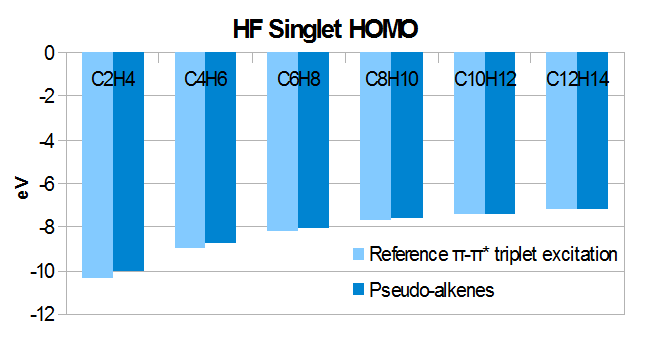
\includegraphics[width=8cm]{hf_homo}
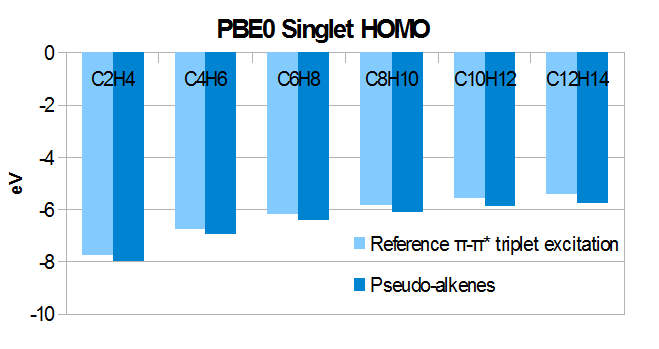
\includegraphics[width=8cm]{pbe0_homo}
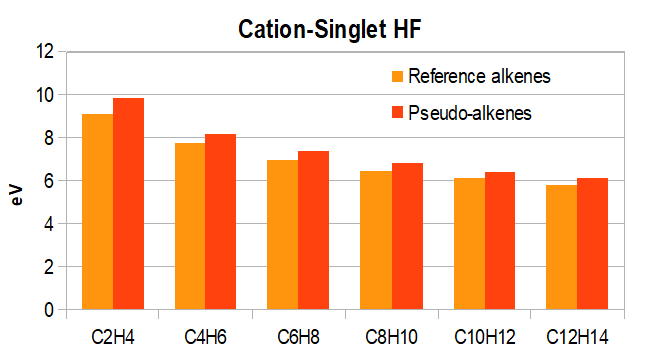
\includegraphics[width=8cm]{hf_ionisation}
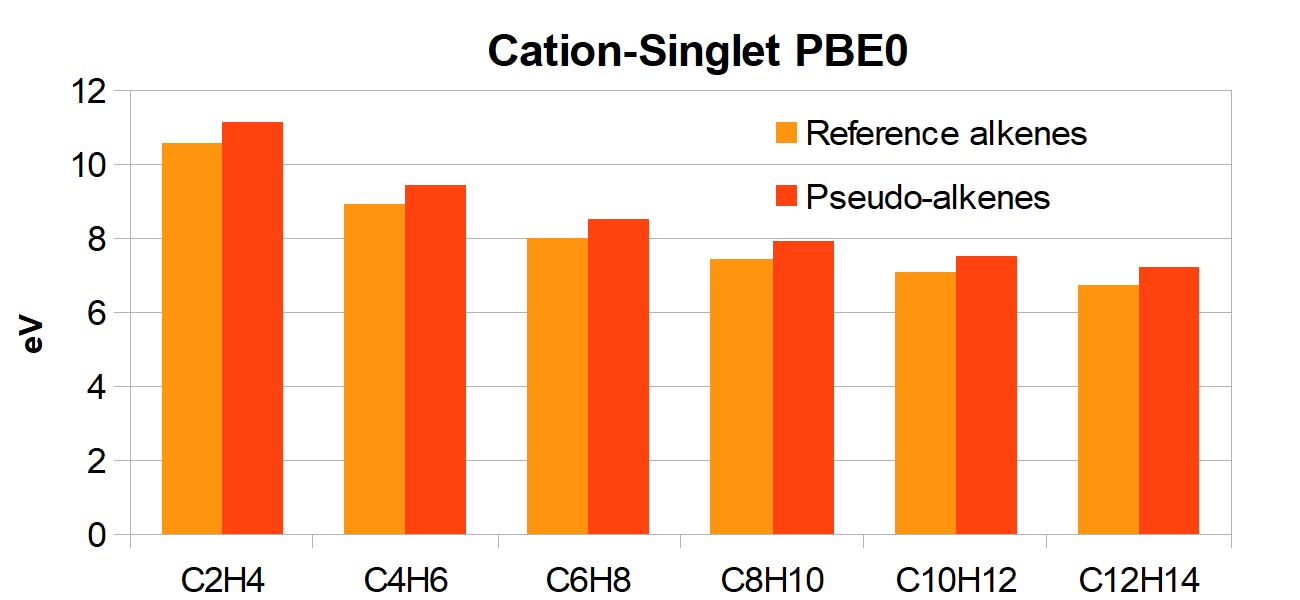
\includegraphics[width=8cm]{pbe0_ionisation}
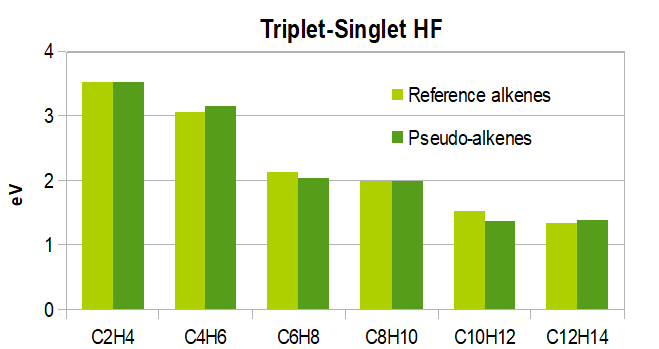
\includegraphics[width=8cm]{hf_excitation}
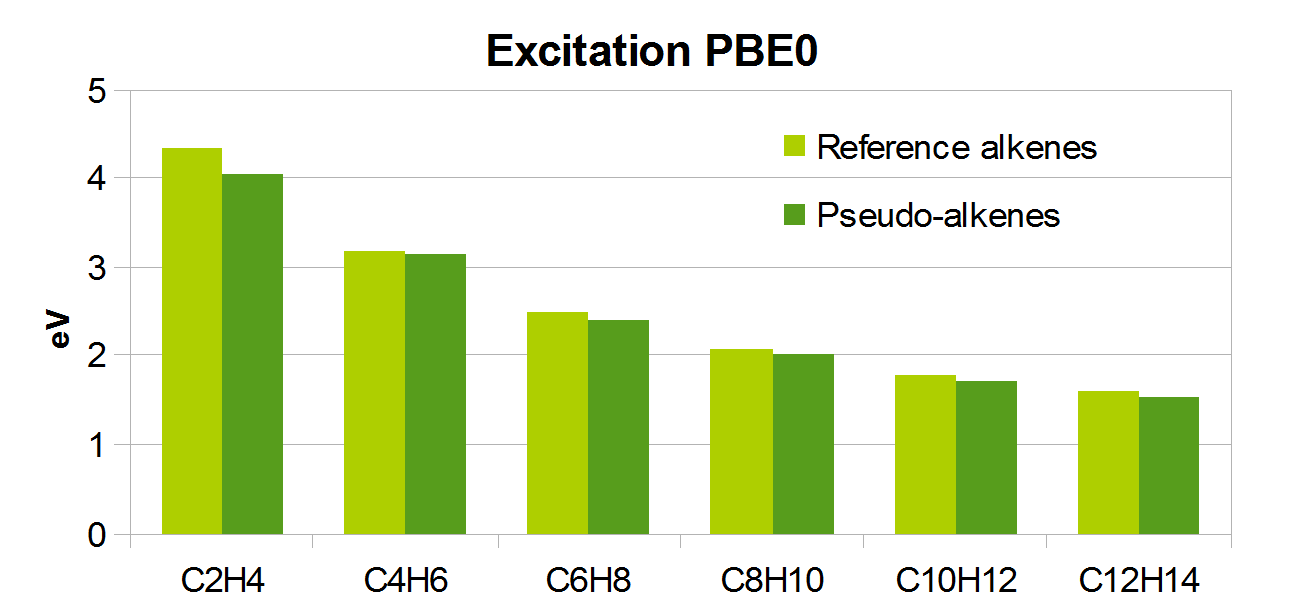
\includegraphics[width=8cm]{pbe0_excitation}
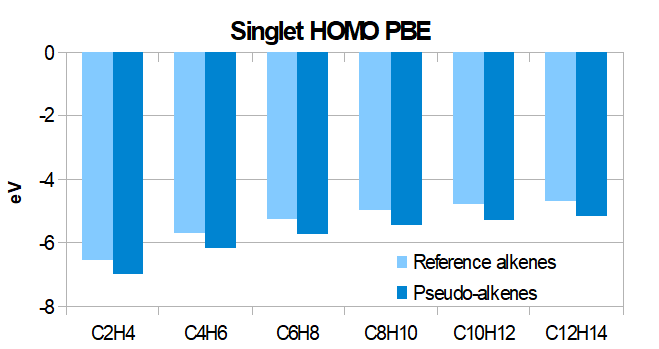
\includegraphics[width=8cm]{pbe_homo}
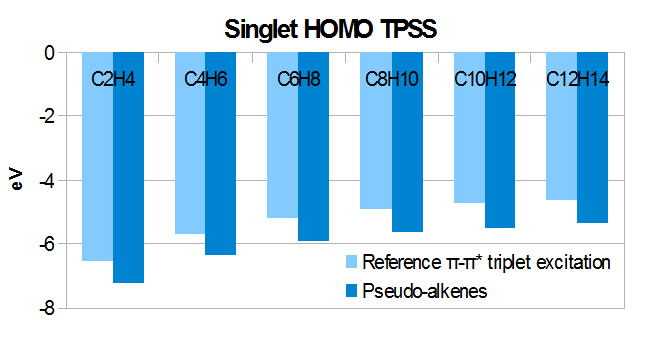
\includegraphics[width=8cm]{tpss_homo}
\end{figure}
\begin{figure}
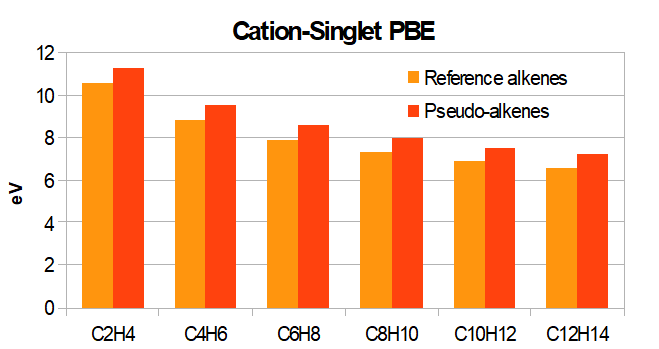
\includegraphics[width=8cm]{pbe_ionisation}
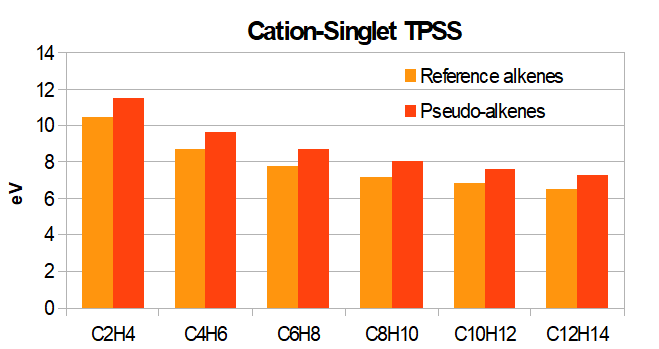
\includegraphics[width=8cm]{tpss_ionisation}
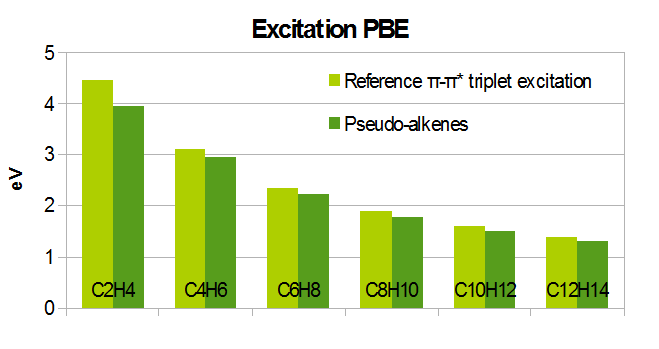
\includegraphics[width=8cm]{pbe_excitation}
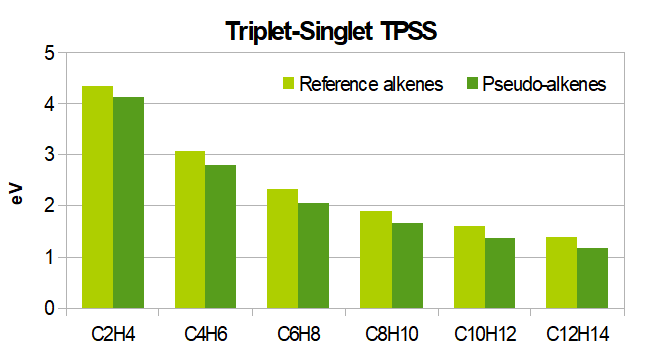
\includegraphics[width=8cm]{tpss_excitation}
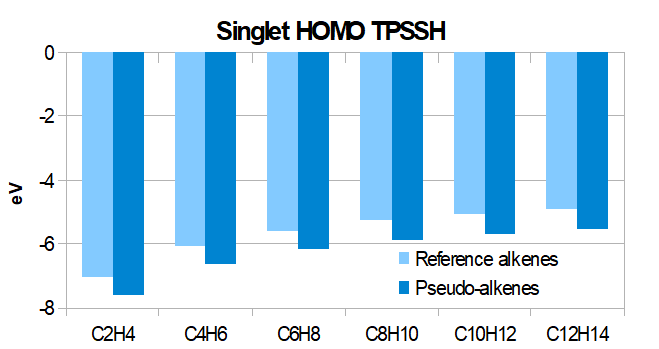
\includegraphics[width=8cm]{tpssh_homo}
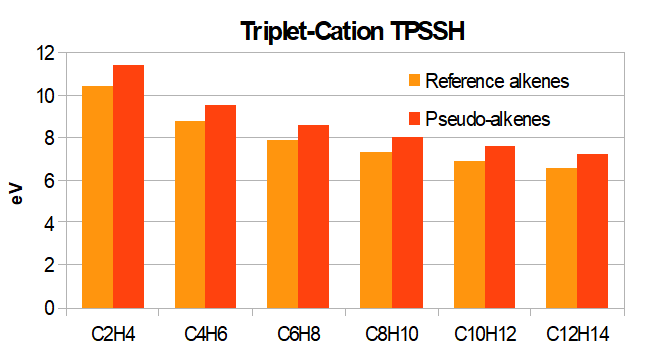
\includegraphics[width=8cm]{tpssh_ionisation}
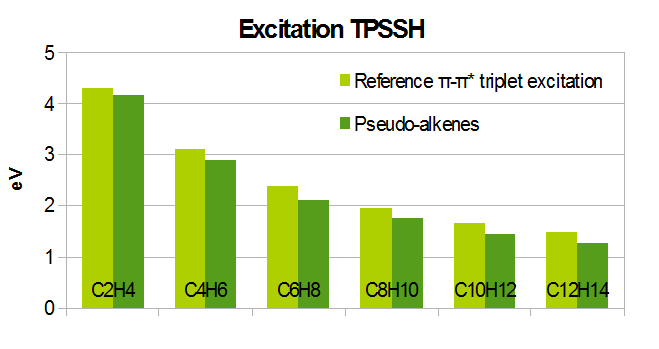
\includegraphics[width=8cm]{tpssh_excitation}
\caption{\%-errors across calculation types for chain alkenes}
\label{fig:alkenes_hf_dft}
\end{figure}
\begin{figure}
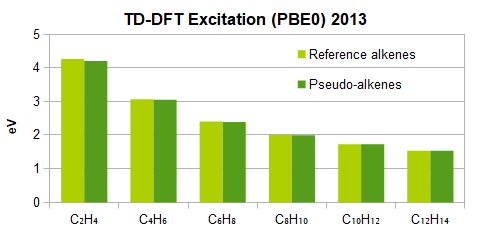
\includegraphics[width=8cm]{tddft_excitation_cd}
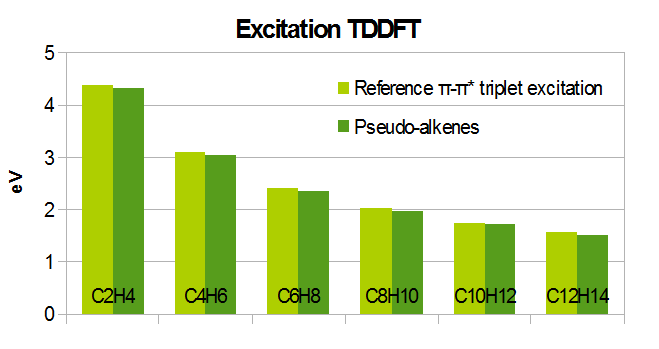
\includegraphics[width=8cm]{tddft_excitation}
\caption{\%-errors across calculation types for chain alkenes}
\label{fig:alkenes_tddft}
\end{figure}

\begin{table}[ht]
\caption{\%-errors across calculation types for chain alkenes}
\begin{tabular}{c c c c c c c}
\hline\hline
Calculation Type & HF & PBE0 & PBE & TPSS & TPSSH & TD-DFT \\
\hline
\(\pi - \pi*\) excitation error (\%) & \(\leq\) 12.5 &\(\leq\) 7.3 & \(\leq\) 12.8 & \(\leq\) 14.1 & \(\leq\) 17.2 & \(\leq\) 2.9 \\
Ionisation error (\%) & \(\leq\) 7.3 & \(\leq\) 6.3 & \(\leq\) 9.0 & \(\leq\) 10.0 & \(\leq\) 9.7 & - \\
Singlet HOMO error (\%) & \(\leq\) 3.0 & \(\leq\) 5.3 & \(\leq\) 9.8 & \(\leq\) 12.1 & \(\leq\) 11.4 & - \\
\hline
\end{tabular}
\label{table:alkene_errors}
\end{table}

\subsection{On Potential-Orbital Overlap}\label{section:po_overlap}

%%%%%%%%%%%%%%%%%%%%%%%%%%%%%%%%%%%%%%%%%%%%%%%%%%%%%%%%%%%%%%%%%%%%%
%% The "Acknowledgement" section can be given in all manuscript
%% classes.  This should be given within the "acknowledgement"
%% environment, which will make the correct section or running title.
%%%%%%%%%%%%%%%%%%%%%%%%%%%%%%%%%%%%%%%%%%%%%%%%%%%%%%%%%%%%%%%%%%%%%
\begin{acknowledgement}

The authors thank \ldots

\end{acknowledgement}

%%%%%%%%%%%%%%%%%%%%%%%%%%%%%%%%%%%%%%%%%%%%%%%%%%%%%%%%%%%%%%%%%%%%%
%% The same is true for Supporting Information, which should use the
%% suppinfo environment.
%%%%%%%%%%%%%%%%%%%%%%%%%%%%%%%%%%%%%%%%%%%%%%%%%%%%%%%%%%%%%%%%%%%%%
\begin{suppinfo}

A listing of the contents of each file supplied as Supporting Information
should be included. For instructions on what should be included in the
Supporting Information as well as how to prepare this material for
publications, refer to the journal's Instructions for Authors.

The following files are available free of charge.
\begin{itemize}
  \item Filename: brief description
  \item Filename: brief description
\end{itemize}

\end{suppinfo}

%%%%%%%%%%%%%%%%%%%%%%%%%%%%%%%%%%%%%%%%%%%%%%%%%%%%%%%%%%%%%%%%%%%%%
%% The appropriate \bibliography command should be placed here.
%% Notice that the class file automatically sets \bibliographystyle
%% and also names the section correctly.
%%%%%%%%%%%%%%%%%%%%%%%%%%%%%%%%%%%%%%%%%%%%%%%%%%%%%%%%%%%%%%%%%%%%%
\bibliography{biblio_pseudo_alex}

\end{document}
